% Subsections 1--2 of the distributed section (input from distributed.tex).

\subsection{Distributed histories}
\label{sec:histories}

A finite set $P$ of \emph{participants} each holds a specification state,
starting at a canonical state $\sigma_S(i_p)$, and changes it only by its own
input and output events.  A participant learns input directly from the
environment or in a message from another participant.  Participants exchange
messages by $\mathsf{send}(m)$ and $\mathsf{receive}(m)$.  A
\emph{message} is a pair $m=(j,d)$ of a cumulative input $j$, or $\varnothing$
if it carries none, and arbitrary other data $d$.  A receive does not change
the specification state; a participant at $(i,R)$ that receives $(j,d)$ with
$j\neq\varnothing$ may incorporate $j$ by its own $\mathsf{input}(k)$ for a
legal common \indesc $k$ of $i$ and $j$, when one exists.

\begin{definition}[Distributed history, consistent cut]
\label{def:distributed-history}
Fix an ordered specification, participants $P$, and an initial input $i_p$
for each.  A \emph{distributed history} $H$ is a finite set of
\emph{history events}, each an occurrence at one participant of an input
event, an output event (Definition~\ref{def:output-event} and
Section~\ref{sec:lifted-output-events}),
$\mathsf{send}(m)$, or $\mathsf{receive}(m)$, with:
\begin{enumerate}
  \item a total local order on each participant's history events;
  \item for each receive, a matching send of the same message at another
        participant, each send matching at most one receive; and
  \item for each participant $p$, its input and output events, in local
        order, form a defined transition sequence from $\sigma_S(i_p)$: each
        is legal at the state where it occurs.
\end{enumerate}
\emph{Happens-before} is the transitive closure of the local orders and of
each send preceding its matching receive.  A \emph{consistent cut} $C$ is a
subset of history events closed under
happens-before~\cite{lamport1978time,chandy1985distributed}; the standard term
is unrelated to our notion of consistency.
\end{definition}

A consistent cut contains a prefix of each participant's history events, so by
item~3
it determines one run per participant.

\begin{definition}[Participant run, endpoint]
\label{def:participant-run}
At a consistent cut $C$, the input and output events of $C$ at participant $p$,
in local order, form its \emph{participant run}, a run
(Definition~\ref{def:run}) whose final state we write $\sigma_p(C)$.  The
\emph{endpoint} of $C$ is $\operatorname{end}(H,C)=(\sigma_p(C))_{p\in P}$.
\end{definition}

\begin{figure}[t]
  \centering
  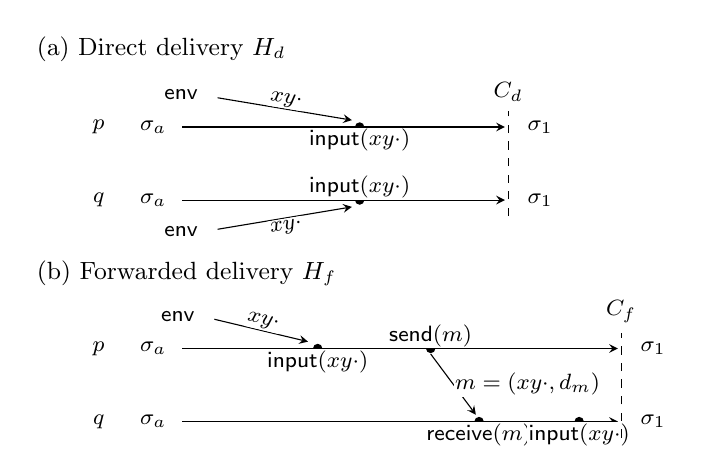
\begin{tikzpicture}[x=.82cm,y=.58cm,>=stealth,
                      every node/.style={font=\footnotesize}]
    % Direct delivery.
    \node[anchor=west,font=\small] at (-1,7.2) {(a) Direct delivery $H_d$};
    \node[anchor=east] at (.35,5.5) {$p$};
    \node[anchor=east] at (.35,3.9) {$q$};
    \node[anchor=west] at (.6,5.5) {$\sigma_a$};
    \node[anchor=west] at (.6,3.9) {$\sigma_a$};
    \draw[->] (1.4,5.5) -- (6.4,5.5);
    \draw[->] (1.4,3.9) -- (6.4,3.9);
    \fill (4.15,5.5) circle (1.7pt);
    \fill (4.15,3.9) circle (1.7pt);
    \node[below,fill=white,inner sep=.5pt] at (4.15,5.5)
      {$\mathsf{input}(xy\cdot)$};
    \node[above,fill=white,inner sep=.5pt] at (4.15,3.9)
      {$\mathsf{input}(xy\cdot)$};
    \node[anchor=east] at (1.8,6.2) {$\mathsf{env}$};
    \node[anchor=east] at (1.8,3.2) {$\mathsf{env}$};
      \draw[->] (1.95,6.14) -- node[midway,above,sloped,fill=white,inner sep=.5pt]
        {$xy\cdot$} (4.03,5.65);
      \draw[->] (1.95,3.26) -- node[midway,below,sloped,fill=white,inner sep=.5pt]
        {$xy\cdot$} (4.03,3.75);
    \draw[dashed] (6.45,3.55) -- (6.45,5.85);
    \node[above] at (6.45,5.85) {$C_d$};
    \node[anchor=west] at (6.6,5.5) {$\sigma_1$};
    \node[anchor=west] at (6.6,3.9) {$\sigma_1$};

    % Forwarded delivery.
    \node[anchor=west,font=\small] at (-1,2.3) {(b) Forwarded delivery $H_f$};
    \node[anchor=east] at (.35,.65) {$p$};
    \node[anchor=east] at (.35,-.95) {$q$};
    \node[anchor=west] at (.6,.65) {$\sigma_a$};
    \node[anchor=west] at (.6,-.95) {$\sigma_a$};
    \draw[->] (1.4,.65) -- (8.15,.65);
    \draw[->] (1.4,-.95) -- (8.15,-.95);
    \node[anchor=east] at (1.75,1.35) {$\mathsf{env}$};
      \draw[->] (1.9,1.29) -- node[midway,above,sloped,fill=white,inner sep=.5pt]
        {$xy\cdot$} (3.35,.8);
    \fill (3.5,.65) circle (1.7pt);
    \node[below,fill=white,inner sep=.5pt] at (3.5,.65)
      {$\mathsf{input}(xy\cdot)$};
    \fill (5.25,.65) circle (1.7pt);
    \node[above,fill=white,inner sep=.5pt] at (5.25,.65)
      {$\mathsf{send}(m)$};
    \fill (6.0,-.95) circle (1.7pt);
    \node[below,fill=white,inner sep=.5pt] at (6.0,-.95)
      {$\mathsf{receive}(m)$};
    \draw[->] (5.25,.53) -- node[midway,right,fill=white,inner sep=.5pt]
      {$m=(xy\cdot,d_m)$} (5.95,-.8);
    \fill (7.55,-.95) circle (1.7pt);
    \node[below,fill=white,inner sep=.5pt] at (7.55,-.95)
      {$\mathsf{input}(xy\cdot)$};
    \draw[dashed] (8.2,-1.3) -- (8.2,1.0);
    \node[above] at (8.2,1.0) {$C_f$};
    \node[anchor=west] at (8.35,.65) {$\sigma_1$};
    \node[anchor=west] at (8.35,-.95) {$\sigma_1$};
  \end{tikzpicture}
  \caption{Two histories from $\sigma_a=\sigma_S(x\cdot\cdot)=(x\cdot\cdot,R_0)$ to
  $\sigma_1=(xy\cdot,R_1)$, with $R_0$ and $R_1$ the tables of
  Figure~\ref{fig:election-frames}(a) and~(b).  In (a) each participant records
  $\mathsf{input}(xy\cdot)$ directly; in (b) $q$ records it after receiving $m$.  Dashed lines are consistent cuts.}
  \label{fig:participant-runs}
\end{figure}

In Figure~\ref{fig:participant-runs}, the input $xy\cdot$ reaches $q$
directly or through a message from $p$.  The histories differ, but at either
cut each participant run is $\mathsf{input}(xy\cdot)$, so both endpoints are
$(\sigma_1,\sigma_1)$.

\subsection{Distributed consistency}
\label{sec:distributed-consistency}

A \emph{continuation} of a history at a consistent cut $C$ is a history $H'$
that extends the history events of $C$ with further history events after
them.  All of $H'$ is a consistent cut of $H'$, its \emph{final cut}.  A
consistent cut $C$ is \emph{confluent at} $j$, for a common \indesc $j$ of
the participants' current inputs, when some continuation at $C$ has a final
cut with endpoint $\bigl((j,R)\bigr)_{p\in P}$ for some $R$: every
participant ends in the same state $(j,R)$.  History events at different
participants are independent, so this holds exactly when the participant runs at $C$ are
confluent at $j$ (Definition~\ref{def:consistency}).

\begin{definition}[Distributed consistency]
\label{def:distributed-consistency}
An ordered specification has \emph{distributed consistency} when, for every
finite participant set, every consistent cut of every history is confluent
at every common \indesc of the participants' current inputs.
\end{definition}

\begin{proposition}[Consistency and distributed consistency]
\label{prop:distributed-consistency}
An ordered specification is consistent if and only if it has distributed
consistency.
\end{proposition}

\begin{proof}[Proof sketch]
The participant runs at a cut are a family of runs, and any family
of runs can be placed at separate participants that exchange no messages.  Full proof in Appendix~\ref{app:proofs-sec4}.
\end{proof}

Both notions are existence claims about transitions
(Section~\ref{sec:scope}).  By Complete CALM,
which reduces to Functional CALM with one output per input, a specification
has distributed consistency exactly when it satisfies Lifted Monotonicity.
For functional specifications,
Corollary~\ref{cor:state-by-input} also gives convergence:

\begin{corollary}[Convergence]
\label{cor:convergence}
In any history of a consistent functional specification, every
participant whose current input at a consistent cut is $j$ is in state
$\sigma_S(j)$.  Participants with the same current input therefore agree,
regardless of message paths, arrival order, or the outputs they emitted.
\end{corollary}

\begin{proof}
Each participant run is a run; apply Corollary~\ref{cor:state-by-input}.
\end{proof}

This is the convergence that strong eventual
consistency~\cite{shapiro2011crdt} asks of replicated state---replicas that
have received the same updates are in equivalent states.  The semilattice merge of CRDTs suffices for it but is not
needed: here it follows directly from any consistent functional specification.  With several outputs per input
this fails even for consistent specifications: in
Figure~\ref{fig:ambiguity-frames}(g), a run that emitted $\{s{\to}\texttt{s1}\}$
has retired the route sets that omit it, while a run at the same input that
emitted nothing keeps them.  Consistency then guarantees that such replicas can
be reconciled, not that they agree.

\paragraph{Message data.}
The data $d$ of a message is any application state other than input that a
participant chooses to send: timestamps, version vectors, non-input-related gossip, votes, etc.  Data
can influence which input and output events occur next at the receiver, but it
never directly changes the receiver's specification state, and nothing in the
definitions above depends on it.  Section~\ref{sec:systems} calls the
rule that makes these choices a participant's \emph{strategy}.  Data can
influence the strategy, but the strategy can decide only within the
specification.
Participants may also share emitted outputs in $d$; this does not change
which cuts are confluent (Appendix~\ref{app:exchanging-outputs}).
